
\begin{table*}[htbp]
  \begin{varwidth}[b]{0.54\linewidth}
    \centering
    \begin{tabular}{rrrr}
    \toprule
    $n$ & brute force & via \cref{alg:blt_pair} & speedup \\
    \midrule
    % Computed here: https://colab.corp.google.com/drive/1_BRrt0jUniaOixKwasKDr7jiSToRwJLj#scrollTo=8tnK5aOnESuk
    2000 & 0.021 & 3.8e-5 & 550$\times$ \\
    20000 & 0.258 & 3.6e-5 & 7176$\times$ \\
    200000 & 4.772 & 4.5e-5 & 104884$\times$ \\
    \bottomrule
    \end{tabular}
    \caption{Seconds to compute $n$ Toeplitz coefficients of $\bfC\inv$. JAX just-in-time (JIT) compilation is \emph{not} included for either approach.}    
    \label{tab:c_inv_coef}
  \end{varwidth} %
  \hfill
  \begin{minipage}[t]{0.44\linewidth}
    \centering
    % Source: https://colab.corp.google.com/drive/1_BRrt0jUniaOixKwasKDr7jiSToRwJLj#scrollTo=e6QNruh2_tBz&uniqifier=1
    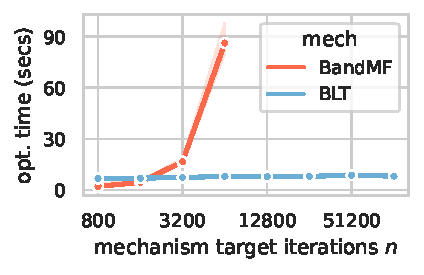
\includegraphics{images/opt_time.pdf} %
    \captionof{figure}{Total wall clock optimization time including JIT compilation on a V100 GPU for \bandmf and \blts, fixing $\minsep=400$ and varying $\nd$. The average over 3 runs is reported.}
    \label{fig:faster}
  \end{minipage}%
\end{table*}


Combining these elements gives us an efficient and differentiable algorithm for computing \maxloss and \rmsloss. Complete pseudo-code for the differentiable loss calculation is given in \cref{alg:blt_loss}. Following \citet{mcmahan2024efficient}, we use auto differentiation and L-BFGS optimizer in JAX~\citep{jax2018github} to optimize $(\theta, \hth)$ for the BLT-DP-FTRL algorithm, and then extract $\bltm(\theta, \omega)$ for noise generation. Similar to \citep{mcmahan2024efficient}, we introduce log-barrier penalties w/ strength $10^{-7}$ to keep $\omega > 0$, $\theta > 0$ and $\theta < 1$ (which is necessary to ensure the Toeplitz coefficients of $\bfC$ are decreasing to satisfy \cref{thm:toepminsepsens}).  
For high precision optimization, we use double precision in JAX on CPUs and GPUs. We observe that increasing buffer size $d$ does not necessarily reduce the loss due to numerical stability and optimization challenges, and different BLT parameter $(\theta, \omega)$ may be achieved in different optimization runs. We also highlight that the different BLT parameters $(\theta, \omega)$ can generate similar Toeplitz coefficients for $\bfC$, which suggests a smaller $d$ might help mitigate the optimization challenge from overparametrization.

The primary motivation for utilizing the $(\theta, \hth)$ parameterization in \cref{alg:blt_loss} is computational efficiency. \cref{tab:c_inv_coef} compares the time to compute $n$ Toepltiz coefficients for $\bfC\inv$ given either $\bltm(\theta, \omega)$ or given $(\theta, \hth$). In the first caes (``brute force''), we construct the Toeplitz coefficients of $\bfC$ using \cref{eq:closedcoefs}, and then solve a linear system (using \texttt{jax.lax.scan} and the property that the inverse of a lower triangular Toeplitz matrix is also lower triangular Toeplitz) to compute the coefficients of $\bfC\inv$). In the second case, we use \cref{alg:blt_pair} to compute $(\omega, \homega)$, and then compute the Toeplitz coefficients by applying \cref{eq:closedcoefs} to $\bltm(\hth, \homega)$. The comparison uses a V100 GPU and a compiled \texttt{jax} implementation, and is repeated many times with an average is given. The second approach can be fully vectorized, and is orders of magnitude faster. This is critical because this is the primary computational step in computing the \rmsloss or \maxloss and occurs in the inner loop of the mechanism optimization procedure: the net result is mechanism optimization is substantially faster than for \bandmf, and scales to much larger $\nd$, see \cref{fig:faster}. \cref{alg:blt_loss} does incur more \texttt{jax} just-in-time (JIT) compilation overhead compared to \bandmf optimization, which accounts \blt optimization being slightly slower for small $\nd$.